% Mindmap
% Author: Stefan Kottwitz
% https://www.packtpub.com/hardware-and-creative/latex-cookbook
\documentclass[border = 60pt]{article}
\usepackage[landscape]{geometry}
\usepackage{scalefnt}
\usepackage{tikz}
\usetikzlibrary{mindmap}
\usetikzlibrary{positioning,calc,arrows,decorations.pathmorphing,intersections,shapes,snakes}
\usepackage{metalogo}
% \usepackage{dtklogos}
\begin{document}
\begin{figure}
  \centering
  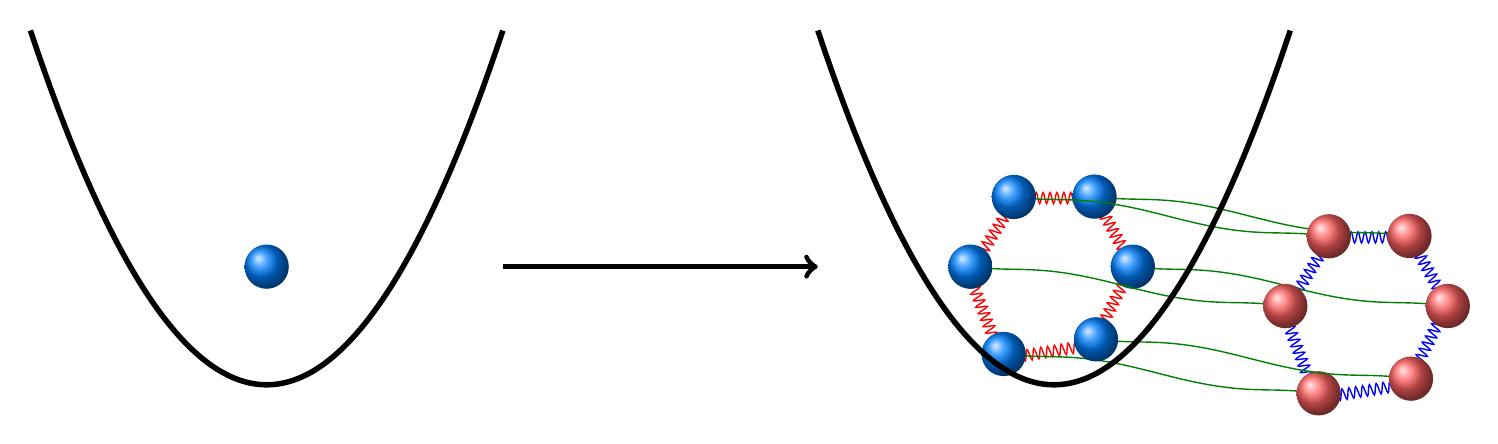
\begin{tikzpicture}
    [
    spring/.style={
      line width=0.5pt, decorate,
      decoration={
        snake, amplitude=2.0, 
        segment length=2.5
      }}, 
    potential/.style={
      line width=0.5pt, decorate,
      color=green!50!black,
      decoration={
        snake, amplitude=2.0, 
        segment length=100
    }}
    ]
    \def\pointsA{
          1.0000/   0.0000,
          0.5136/   0.8896,
         -0.5112/   0.8853,
         -1.0629/   0.0000,
         -0.6401/  -1.1086,
          0.5326/  -0.9226
    }
    \def\rpoffset{(4.0, -0.5)}

    % First, draw the springs for the first RP
    \draw[spring, color=red] (  1.0000,   0.0000) 
                          -- (  0.5136,   0.8896) 
                          -- ( -0.5112,   0.8853) 
                          -- ( -1.0629,   0.0000) 
                          -- ( -0.6401,  -1.1086) 
                          -- (  0.5326,  -0.9226) 
                          -- cycle;
    % First, draw the springs for the second RP
    \draw[spring, color=blue] ($ (  1.0000,   0.0000) + (4.0, -0.5) $)
                          -- ($ (  0.5136,   0.8896) + (4.0, -0.5) $)
                          -- ($ ( -0.5112,   0.8853) + (4.0, -0.5) $)
                          -- ($ ( -1.0629,   0.0000) + (4.0, -0.5) $)
                          -- ($ ( -0.6401,  -1.1086) + (4.0, -0.5) $)
                          -- ($ (  0.5326,  -0.9226) + (4.0, -0.5) $)
                          -- cycle;

    % Draw the single particles
    \shade[shading=ball, ball color=blue!50!cyan] (-10, 0) circle (8pt);

    \foreach \x/\y in \pointsA {
      \coordinate (A) at (\x, \y);
      % draw the interaction between the two atoms
      \draw[potential] (A) -- ++\rpoffset;
      % Ring-Polymer of the first atom
      \shade[shading=ball, ball color=blue!50!cyan] (A) circle (8pt);
      % Ring-Polymer of the second atom
      \shade[shading=ball, ball color=red!50!pink] ($ (A) + (4.0, -0.5) $) circle (8pt);
    }

     % Draw the potential
     \draw [line width=2pt, domain=-13:-7] plot [samples=300] (\x, {0.5 * (\x + 10) * (\x + 10) - 1.5});
     \draw [line width=2pt, domain=-3:3] plot [samples=300] (\x, {0.5 * (\x + 0) * (\x + 0) - 1.5});
     % Draw an arrow
     \draw [line width=2pt, ->] (-7, 0) -- (-3, 0);
  \end{tikzpicture}
\end{figure}

\begin{figure}
  \centering
  \resizebox{\textwidth}{!}{
    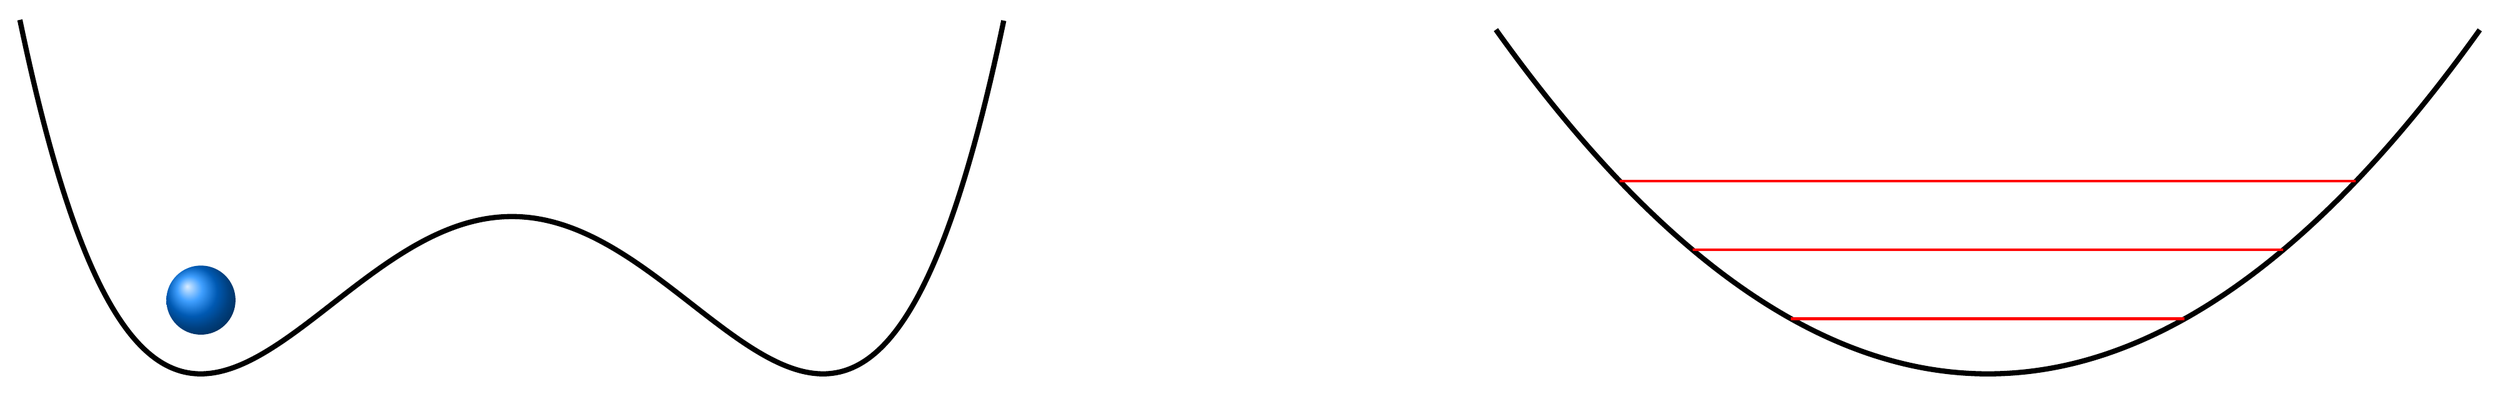
\begin{tikzpicture}
        % [scale=0.4, transform shape]
        % Draw the potentials
        \draw [line width=3pt, domain=20:40] plot [samples=300] (\x, {0.07 * (\x - 30) * (\x - 30)});
        \draw [line width=3pt, domain=-10:10] plot [samples=300] (\x, {(\x*\x*\x*\x - 80*\x*\x + 1600) / 500});
        % draw the quantization of energy levels
        \draw [line width=1.5pt, color=red] (26, 1.12) -- (34, 1.12);
        \draw [line width=1.5pt, color=red] (24, 2.52) -- (36, 2.52);
        \draw [line width=1.5pt, color=red] (22.52, 3.92) -- (37.48, 3.92);
        % draw the particles
        \shade[ball color=blue!50!cyan] (-6.32, 1.5) circle (20pt);
        % annotatons
        % \node at (0, -2) {\fontsize{72pt}{12pt}\selectfont Quantum Tunneling};
        % \node[] at (30, -2) {\Huge Zero Point Motion};
    \end{tikzpicture}
  }
\end{figure}
\end{document}

%%% Local Variables:
%%% mode: latex
%%% TeX-master: t
%%% End:
